\section{x86}

\subsection{MSVC}

Here is what we get after compilation (MSVC 2010 Express):

\lstinputlisting[label=src:passing_arguments_ex_MSVC_cdecl,caption=MSVC 2010 Express]{patterns/05_passing_arguments/msvc_EN.asm}

\myindex{x86!\Registers!EBP}

What we see is that the \main function pushes 3 numbers onto the stack and calls \TT{f(int,int,int).} 

Argument access inside \ttf is organized with the help of macros like: \TT{\_a\$ = 8}, 
in the same way as local variables, but with positive offsets (addressed with \IT{plus}).
So, we are addressing the \IT{outer} side of the \gls{stack frame} by adding the \TT{\_a\$} macro to the value in the \EBP register.

\myindex{x86!\Instructions!IMUL}
\myindex{x86!\Instructions!ADD}

Then the value of $a$ is stored into \EAX. After \IMUL instruction execution, the value in \EAX is 
a \gls{product} of the value in \EAX and the content of \TT{\_b}.

After that, \ADD adds the value in \TT{\_c} to \EAX.

The value in \EAX does not need to be moved: it is already where it must be.
On returning to \gls{caller}, it takes the \EAX value and use it as an argument to \printf.

\subsection{MSVC + \olly}
\myindex{\olly}
Let's illustrate this in \olly.
When we trace to the first instruction in \ttf that uses one of the arguments 
(first one), we see that \EBP is pointing to the \gls{stack frame}, 
which is marked with a red rectangle.

The first element of the \gls{stack frame} is the saved value of \EBP, 
the second one is \ac{RA}, the third is the first function argument, then the second and third ones.

To access the first function argument, one needs to add exactly 8 (2 32-bit words) to \EBP.

\olly is aware about this, so it has added comments to the stack elements like

\q{RETURN from} and \q{Arg1 = \dots}, etc.

N.B.: Function arguments are not members of the function's stack frame, they are rather
members of the stack frame of the \gls{caller} function.

Hence, \olly marked \q{Arg} elements as members of another stack frame.

\begin{figure}[H]
\centering
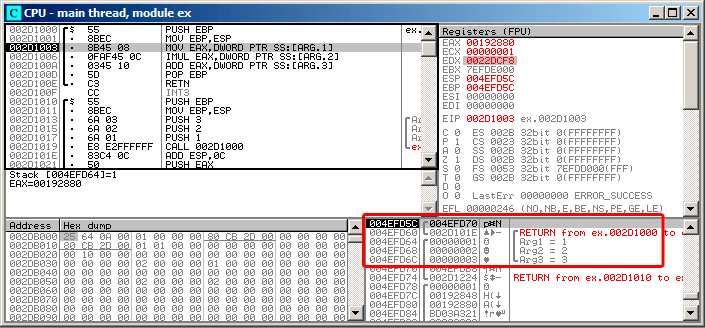
\includegraphics[scale=\FigScale]{patterns/05_passing_arguments/olly.png}
\caption{\olly: inside of \ttf{} function}
\label{fig:passing_arguments_olly}
\end{figure}



\subsection{GCC}

Let's compile the same in GCC 4.4.1 and see the results in \IDA:

\lstinputlisting[caption=GCC 4.4.1]{patterns/05_passing_arguments/gcc_EN.asm}

The result is almost the same with some minor differences discussed earlier.

The \gls{stack pointer} is not set back after the two function calls(f and printf), 
because the penultimate \TT{LEAVE} (\myref{x86_ins:LEAVE}) 
instruction takes care of this at the end.
